\documentclass[9pt]{beamer}

\geometry{paperwidth=213.3mm,paperheight=120mm}

\usetheme[{titleformat plain}=smallcaps,
           titleformat title=smallcaps,
           titleformat subtitle=regular,
           titleformat section=smallcaps,
           titleformat frame=smallcaps,
           % numbering=fraction,
          ]{metropolis}
% \usepackage{appendixnumberbeamer}

\definecolor{mLightGreen}{HTML}{14B03D}
\definecolor{vpGreen}{HTML}{66c2a5}
\definecolor{vpOrange}{HTML}{fc8d62}
\providecommand{\iRef}[1]{{\color{mLightGreen}\small $[$#1$]$}}

\usepackage{booktabs}
\usepackage[scale=2]{ccicons}

\usepackage{../_style/common}
\usepackage{../_style/defs}

\usepackage{tikz}
\usetikzlibrary{shapes,arrows}
\usepackage{amsmath, bm}
\usepackage{siunitx}
\usepackage{physics,hepnames}
\usepackage{mathtools}
\usepackage{enumitem}
\setenumerate[1]{%
      label=\protect\usebeamerfont{enumerate item}%
      \protect\usebeamercolor[fg]{enumerate item}%
      \insertenumlabel.}
\setitemize{label=\usebeamerfont*{itemize item}%
    \usebeamercolor[fg]{itemize item}
      \usebeamertemplate{itemize item}}

\usepackage{subfig}
\usepackage{colortbl}
\usepackage{multirow}
\usepackage{pifont}

\usepackage{pgfplots}
\usepgfplotslibrary{dateplot}

\usepackage{ulem}

\graphicspath{{pictures/}}

\title{PDF sampling}
\subtitle{as \sout{Bayesian} na\"ive as possible}
\date{August, 2022}
\author{\textit{\textbf{Alessandro Candido}}, Luigi Del Debbio, Tommaso Giani, Giacomo Petrillo}
%\institute{N3PDF}
\titlegraphic{
    \raisebox{10pt}[0pt][0pt]{
\includegraphics[width=2.5cm]{../_logos/nnpdf_logo.pdf}}\hspace*{10pt}
    \hfill
    \raisebox{5pt}[0pt][0pt]{
\includegraphics[height=0.8cm]{../_logos/n3pdf_logo.pdf}}\hspace*{10pt}
    
\includegraphics[height=1.3cm]{../_logos/erc_logo1.png}

    \vfill\vspace*{230pt}
    
\includegraphics[height=1cm]{../_logos/unimi_logo.png}\hfill
    
\includegraphics[height=1cm]{../_logos/infn_logo.png}\\
    \vspace*{5pt}
    {
        \fontsize{3pt}{3.5pt}\selectfont
        \begin{center}
            This project has received funding from the European Union's Horizon
            2020 research and innovation programme under grant agreement No
            740006\quad 
\includegraphics[height=5pt]{../_logos/eu-flag.jpg}
        \end{center}
    }
}

\begin{document}

\maketitle

\setlist[description]{font=\quad\normalfont\bfseries\scshape\space}
\metroset{block=fill}

\section{Fitting functions 101}

\begin{frame}{Function space}
    \begin{columns}
        \begin{column}{0.5\textwidth}
            A function $f: \mathbb{R} \to \mathbb{R}$ (or suitable intervals)
            lives in a infinite-dimensional space.
            \vspace*{20pt}

            This has a simple consequence:
            \begin{block}{Under-determination}
                Fitting an \textbf{unknown function} on a finite number of data
                is always an \textbf{under-determined} problem.
            \end{block}
            \vspace*{20pt}

            How to choose a solution, when \alert{many} are available and
            \alert{equivalent}?
        \end{column}
        \begin{column}{0.5\textwidth}
            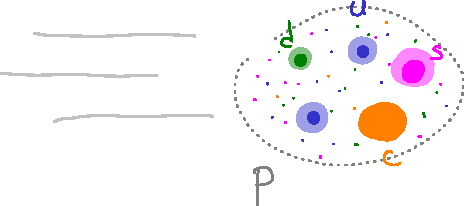
\includegraphics[width=\textwidth]{intrinsic}
        \end{column}
    \end{columns}
\end{frame}

\begin{frame}{Solutions in the Assumptions}
    cut

    regularize
\end{frame}

\begin{frame}{So Which?}
    Then which one should we choose?

    There is not an absolute best answer, because both procedures might be arbitrary.
    According to me, the principle to follow is "choose that convey more
    physical insight" in such a way to trade physical assumptions for arbitrariness.
\end{frame}

\begin{frame}{The NN}
    What is then doing the neural network (NN)? Why is it working so well?

    First: "working" is ambiguous, because we don't know the answer. Closure
    tests are a clue, but we want something to perform well on the truth, and
    not knowing it we are extrapolating from something that is working well on
    a truth candidate.

    Second: interpolation assumption in the training.
\end{frame}

\begin{frame}{Looking for Insights}
    NNPDF methodology has many good things:
    - nice representation of a generic distribution (replicas)
    - many tests in place
    - fast theory
    - lots of data

    We don't want to give up on any of these.

    ---

    On the other hand, a pain point is the insight we have on the
    representation itself: we trust on it because of tests, but it is sometimes
    difficult to pin down results to features.

    \begin{exampleblock}{Hopscotch}
        There are some physical assumptions we can check:
        - integrability and sum rules
        - positivity
        - t0 chi2

        But the result might be more subtle: might be hidden in regularization.
    \end{exampleblock}
\end{frame}

\begin{frame}{Restart from Bayes}
    Typical examples of ML are image and speech recognition, generative tasks,
    style transfer and so on.

    All these problems have in common very high dimensional objects, with poor
    analytical insight on its structure. Working out an explicit and effective
    representation for them is difficult.

    This is not the case of PDF: we already describe them with a math language,
    and we have clear analytic properties at hand (sum rules, power-like
    behavior, and so on).
    
    ---

    Then, (Bayes).

    \begin{equation*}
        P(A|B) = \frac{P(B|A) P(A)}{P(B)}
    \end{equation*}
    
    Advantage: an explicit prior will do what the NN is now doing.
\end{frame}

\begin{frame}{Prior Choice \& Implementation}
    Gaussian process
    
    ---

    Fit Basic idea: take a bunch of points out of the function, the rest comes
    by interpolation. Which ones? LHAPDF's of course :)
\end{frame}


\begin{frame}{(Very) Preliminary Results}
\end{frame}

\begin{frame}[standout]
    Questions?
\end{frame}

\appendix

\begin{frame}{PDF features}
    \begin{description}
        \item[sum rules] analytically, zero errors data point on the primitive
        \item[quadratic points] least square fit
        \item[PDF positivity] we can fit the log processes
    \end{description}
\end{frame}

\begin{frame}{Further results}
\end{frame}

\end{document}
